%!TEX root = main.tex

\chapter{Estado del arte}
El proyecto Bio2RDF utiliza las tecnologías de la web semántica para su
implementación y funcionamiento. Así, el análisis que se hará en esta memoria
toma estos conocimientos como base y generará a través de ellos estadísticas de
centralidad con las cuales se determinará cuales son los datos más importantes
de dicha base de datos.

Para poder analizar el problema correctamente es necesario el conocimiento de
las tecnologías que se enuncian en este capítulo. En la sección \ref{ea:ws} se
describe qué es la web semántica y las tecnologías que la componen.
En la sección \ref{ea:bio} se hace una revisión al proyecto Bio2RDF y a las
bases de datos que forman parte de él, en especial a la utilizada en este
documento: DrugBank; y en la sección \ref{ea:cent} se repasan conceptos básicos
de teoría de grafos y se introduce el concepto de centralidad junto a sus
métricas y algoritmos.

\section{Web Semántica}\label{ea:ws}
La web semántica es un conjunto de actividades propuestas por la \emph{World
Wide Web Consortium} (desde ahora W3C) con el objetivo de generar tecnologías
para la publicación de datos en la web de tal manera que sean procesables por
las maquinas. 
Se basa en la idea de añadir metadatos semánticos y ontológicos que describan el
contenido y la relación entre los datos publicados. De esta manera se logra
mejorar la interoperatividad de internet pues los programas podrán acceder a los
datos en un lenguaje formal, procesar su contenido, razonar en base a este y
combinarlo para resolver problemas cotidianos automáticamente.

Es posible rastrear los orígenes de esta idea hasta una propuesta temprana de la
\emph{world wide web} en 1986~\cite{berners1989proposal} y el subsecuente
trabajo de Berners-Lee \etal\cite{berners1992world} donde se prevé la
necesidad de una evolución desde objetos legible por las personas a información
semántica orientada a las máquinas.

Para lograr los objetivos de la web semántica se han generado múltiples
metalenguajes y estándares de representación como son XML, XML Schema, RDF,
RDF Schema, OWL y SPARQL. Estas tecnologías se utilizan actualmente para generar
datos enlazados (\emph{Linked Data}), que buscan enlazar información arbitraria
en la web generando así una ``\emph{red de las cosas del mundo, descrita por los
datos en la Web}''\cite{berners2011linked}.

\begin{figure}[htpb]
  \centering
  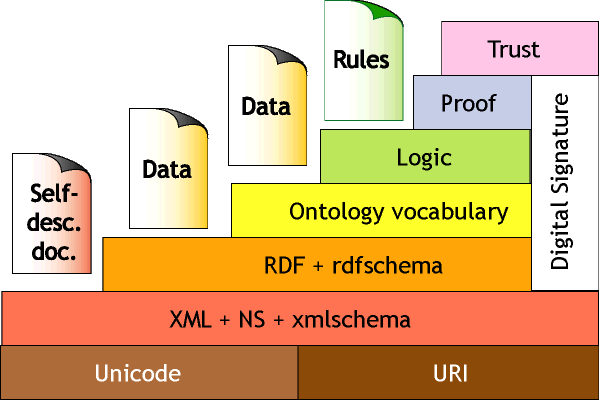
\includegraphics[width=.6\textwidth]{figures/Semantic_web_stack.png}
  \caption{Pila de tecnologías de la web semántica.}
  \vspace{-.25cm}
  \caption*{Creado por Marobi1\cite{wikimg:swstack}.}
  \label{fig:swstack}
\end{figure}

En las siguientes secciones se describirán más detalladamente algunos de los
conceptos presentados en la figura \ref{fig:swstack} comenzando desde la base,
con las tecnologías del hipertexto (URI y XML), para luego pasar a las
tecnologías de la web semántica más estandarizadas (RDF, RDFS y OWL) y terminar
con el lenguaje de consulta SPARQL.

\subsection{URI}
Una URI (del las siglas del ingles \emph{Uniform Resource Identifier}) es una
cadena de caracteres utilizada para identificar un recurso inequívocamente.
Si bien en un principio solo acepta un subconjunto caracteres ASCII (el alfabeto
en ingles y los números) y ``código porciento'' (en el cual, por ejemplo '\%26'
es '\&') el estándar fue extendido el 2005 a IRI (\emph{Internationalized
resource identifier}) que puede contener caracteres Unicode/ISO 10646,
incluyendo chino, japones, koreano, entre otros\cite{gangemi2006bourne}.
En este documento no se diferenciará entre URI e IRI.

La sintaxis actual de una URI fue definida por Berners-Lee et al. el
2005 ~\cite{berners2004uniform} como sigue:\\
\texttt{
  scheme:{[//{[user:passwd@]}host{[:port]}]}{[/]}path{[?query]}{[\#frag]}
}\\
donde:
\begin{itemize}
  \item
    El \bf{esquema} (\emph{scheme}) que consiste en una secuencia de caracteres
    sensibles a las mayúsculas que comienza con una letra y es seguido por
    cualquier combinación de letras, puntos (\tt{.}), guiones (\tt{-}) y signos
    más (\tt{+}), terminando con dos puntos (\tt{:}). 
    Ejemplos populares son \tt{http:}, \tt{ftp:} y \tt{mailto:}.
  \item
    Las dos barras (\tt{//}) son requeridos para algunos esquemas. Cuando la
    componente de autoridad no está presente la ruta no puede comenzar con dos
    barras.
  \item
    La \bf{autoridad} se divide como sigue:
    \begin{itemize}
      \item
        Una \bf{autentificación} opcional compuesta por el usuario
        (\emph{user}), dos puntos y una contraseña (\emph{password}) terminando
        en un arroba (\tt{@}).
      \item
        Un anfitrión (\emph{host}) que puede ser un nombre registrado un una
        dirección IP.
      \item
        Un número de \bf{puerto} opcional (\emph{port}) separado del anfitrión
        por dos puntos.
    \end{itemize}
  \item
    Una \bf{ruta} (\emph{path}) que es una secuencia de segmentos separados
    por una barra (\tt{/}) que comienza con una de las mismas. Generalmente
    representa la localización de un archivo en un sistema de archivos
    jerárquico pero no es necesario.
  \item
    Una \bf{consulta} opcional (\emph{query}) que comienza con un signo de
    interrogación (\tt{?}) y, a pesar de no tener un sintaxis claramente
    definida, usualmente presenta pares atributo-valor.
  \item
    Un \bf{fragmento} opcional (\emph{fragment}) que comienza con un numeral
    (\tt{\#}) seguido por un identificador secundario al recurso principal.
\end{itemize}

\begin{figure}[htpb]
  $$
    \underbrace{\text{http}}_{\text{esquema}}\text{://}
    \overbrace{
      \overbrace{
        \underbrace{\text{user:password}}_{\text{autentificación}}\text{@}
        \underbrace{\text{example.com}}_{\text{anfitrión}}\text{:}
        \underbrace{\text{80}}_{\text{puerto}}
      }^{\text{autoridad}}
      \overbrace{\text{/path/data}}^{\text{ruta}}
    }^{\text{parte jerárquica}}\text{?}
    \underbrace{\text{key=value}}_{\text{consulta}}\text{\#}
    \underbrace{\text{section1}}_{\text{fragmento}}
  $$
  \caption{Ejemplo de una URI.}
  \label{fig:uriex}
\end{figure}

Un ejemplo de lo anterior sería la figura \ref{fig:uriex} donde podemos notar
que una URL (\emph{Uniform Resource Locator}) es una URI, pero no debemos
confundir los términos pues una URL además de identificar un recurso web permite
obtener una representación del mismo generalmente en formato HTML vía HTTP. Es
decir, una URL es una URI que apunta a un recurso físico en la web, mientras que
una URI no necesariamente debe apuntar a una localización que exista realmente.

\subsection{XML}
XML es el acrónimo del ingles \emph{Extensible Markup Language}. Es un
lenguaje de marcas desarrollado por el W3C para almacenar datos de manera
legible tanto por personas como por máquinas. 
El diseño de XML busca la simplicidad, generalidad y usabilidad a través de
internet\cite{paoli2004extensible}. 

Un documento XML puede comenzar con un identificador declarando alguna
información sobre el documento en sí. Luego el cuerpo del fichero debe contener
solo un elemento raíz y dentro de éste se pueden escribir múltiples elementos y
atributos.

\begin{figure}[htpb]
  \centering
  \begin{tabular}{c}
    \lstinputlisting[
      basicstyle=\ttfamily\scriptsize,
      language=xml]{code/example-xml.xml}
  \end{tabular}
  \caption{Ejemplo de XML.}
  \vspace{-.25cm}
  \label{fig:xmlex}
\end{figure}

En la figura~\ref{fig:xmlex} vemos la libertad que nos da XML a la hora de
representar cualquier tipo de información, pero esta libertad hace que
interpretar la validez de un documento sea complicado, pues la información
contenida en este puede ser sensible a la aplicación y el lenguaje definido con
esta tecnología. En respuesta a esta problemática el W3C desarrolló \emph{XML
Schema} que cobra vital importancia para la web semántica.

\subsection{XSD}
XSD (del ingles \emph{XML Schema Definition}) es una recomendación del W3C que
especifica formalmente la estructura y restricciones de los contenidos de un
fichero XML de manera precisa más allá de las normas sintácticas del propio
lenguaje XML.

A diferencia de otros lenguajes de esquemas para XML, XSD especifica también
tipos de datos y sus restricciones, logrando un estándar a la hora de
representar datos~\cite{biron2004xml}. 
Presenta 19 tipos de datos básicos: \tt{anyURI},
\tt{base64Binary}, \tt{boolean}, \tt{date}, \tt{dateTime}, \tt{decimal},
\tt{double}, \tt{duration}, \tt{float}, \tt{hexBinary}, \tt{gDay}, \tt{gMonth},
\tt{gMonthDay}, \tt{gYear}, \tt{gYearMonth}, \tt{NOTATION}, \tt{QName},
\tt{string} y \tt{time}. Además permite la creación de nuevos tipos de datos por
medio de tres mecanismos:
\begin{itemize}
  \item \bf{Restricción:} Reduce los valores que puede tomar un dato.
  \item \bf{Lista:} Permite una secuencia de valores.
  \item \bf{Unión:} Permite la elección de valores de diferentes tipos.
\end{itemize}

Gracias a estos factores un fichero XML Schema puede representar un modelo de
datos completo y robusto, con relaciones entre las entidades y asignaciones de 
tipos de datos básicos. La figura~\ref{fig:xsdex} muestra un ejemplo del uso de
XML en conjunto con XSD.

Esta característica es fundamental para la web semántica pues todos los tipos de
datos de XSD son compatibles con RDF.

\begin{figure}[htpb]
  \centering
  \begin{tabular}{c}
    \lstinputlisting[
      basicstyle=\ttfamily\scriptsize,
      language=xml]{code/example-xmls.xml}
  \end{tabular}
  \caption{Ejemplo de XMLS.}
  \vspace{-.25cm}
  \caption*{Definiendo una película con XSD.}
  \label{fig:xsdex}
\end{figure}

\subsection{RDF}
RDF (del inglés \emph{Resource Description Framework}) es una familia de
especificaciones del W3C diseñada como un modelo de datos para metadatos.
Fue adoptado como una recomendación del W3C en 1999, mientras que la
especificación 1.0 fue publicada el 2004 y la 1.1 el
2014\cite{bikakis2013semantic}.

El modelo de datos RDF se basa en la idea de hacer declaraciones sobre 
recursos web (URIs) en forma de expresiones $\langle sujeto, predicado, objeto
\rangle$ que son llamados triples RDF.
El $sujeto$ indica el recurso mientras que el $predicado$ denota la relación
con el $objeto$.
Digamos $U$ un conjunto de URIs, $B$ un conjunto de recursos anónimos y $L$ un
conjunto de literales XSD, podemos denotar un triple RDF como 
$\langle s,p,o\rangle \in (U\cup B) \times U \times (U\cup B\cup L)$.
Así podemos decir que un triple RDF sigue la clásica notación \tt{entidad} - 
\tt{atributo} - \tt{valor} de los modelos orientados a objetos, permitiendo
además, gracias a su simpleza, modelar todo tipo de conceptos abstractos.

Llamaremos vocabulario a la definición de conceptos y relaciones (términos)
utilizados para describir y representar un área de conocimiento.
Otro concepto a tener en cuenta son las ontologías, aunque no existe una clara 
división entre éstas y los vocabularios, generalmente se les considera más
complejas y formales.
En la web semántica una colección de triples RDF puede denotar un vocabulario o
ontología.

El vocabulario incluido en la especificación RDF es muy básico y por ello fue
extendido a \emph{RDF Schema}, por lo que la gran mayoría de las bases de datos
RDF actuales contienen ambos vocabularios.

Un conjunto de triples RDF será representado naturalmente por un grafo dirigido.
Esta característica faculta la tecnología para ser parte fundamental de la web 
semántica pues permite relacionar información de diferentes fuentes sin mayor
problema y representarla en un esquema fácilmente identificable.

RDF es un modelo abstracto con varios formatos de serialización, por lo que la
codificación de un triple varía dependiendo el tipo de archivo en el que se
guarde. En esta memoria se trabajará con triples codificados en RDF/XML,
Turtle\cite{beckett2014turtle} y N-Triples\cite{beckett2014nt}.

RDF/XML fue la primera codificación estándar para serializar RDF (en un archivo
XML) y si bien es potente, es difícil de leer por las personas. En base a esto
utilizaremos Turtle y N-Triples pues su simpleza los hace ideales para el
entendimiento y procesamiento de los triples.

Algunas de las reglas para escribir un archivo Turtle (\tt{.ttl}) son las
siguientes:
\begin{itemize}
  \item Toda sentencia termina con un punto (\tt{.}).
  \item La sucesión de tres URIs es un triple.
  \item 
    Si una linea termina en punto y coma (\tt{;}) la siguiente linea mantiene el
    $sujeto$ y solo es necesario escribir las URIs del $predicado$ y el
    $objeto$.
  \item 
    Se pueden definir prefijos con \tt{@prefix rdf: <some\_URI> .}. Esta
    característica es particularmente útil para agregar vocabularios ya
    definidos.
\end{itemize}

N-Triples es una subsección del lenguaje Turtle y su característica principal es
la facilidad que presenta a la hora de analizar su sintaxis. En un archivo
N-Triples (\tt{.nt}) solo se pueden escribir tres URIs seguidas de un punto para
representar un triple RDF y todo lo que esté después de un numeral (\tt{\#}) se
considera un comentario.

Podemos encontrar una descripción completa de las características y sintaxis de
Turtle en~\cite{beckett2014turtle}, de N-Triples en~\cite{beckett2014nt} y de
RDF/XML en ~\cite{beckett2004rdf}.

En la figura \ref{fig:triples} podemos ver un ejemplo básico de la utilización 
de Turtle para la generación de triples (figura \ref{fig:triples:ttl}), el
mismo ejemplo escrito en XML/RDF (figura \ref{fig:triples:rdf}) y como estos
pueden ser visualizados como un grafo dirigido (\ref{fig:triples:grafo}).
\begin{figure}[htpb]
  \centering
  \begin{subfigure}[b]{\textwidth}
    \centering
    \begin{tabular}{c}
      \lstinputlisting[basicstyle=\ttfamily\scriptsize]{
        code/example-turtle.ttl}
    \end{tabular}
    \caption{Ejemplo en Turtle.}
    \label{fig:triples:ttl}
  \end{subfigure}
  \\[0.5cm]
  \begin{subfigure}[b]{\textwidth}
    \centering
    \begin{tabular}{c}
      \lstinputlisting[basicstyle=\ttfamily\scriptsize]{
        code/example-xml-rdf.rdf}
    \end{tabular}
    \caption{Mismo ejemplo en XML/RDF.}
    \label{fig:triples:rdf}
  \end{subfigure}
  \\[0.5cm]
  \begin{subfigure}[]{\textwidth}
    \centering
    \begin{tikzpicture}
  \begin{scope}[every node/.style={ellipse,thick,draw,font=\small}]
    \node (A) at (0,0)    {ex:utfsm};
    \node (B) at (6,1.5)  {ex:universidad};
    \node (C) at (6,0)    {ex:federico};
    \node (D) at (6,-1.5) {http://www.usm.cl};
    \node (E) at (12.5,0) {Federico Santa Maria};
  \end{scope}
  \begin{scope}[>={Stealth[black]},
                every node/.style={font=\footnotesize},
                every edge/.style={draw=black,very thick}]
    \path[->] (A) edge [sloped, above]   node {rdf:type}      (B);
    \path[->] (A) edge [above]           node {ex:fundador}   (C);
    \path[->] (A) edge [sloped, below]   node {ex:pagina}     (D);
    \path[->] (C) edge [above, pos=0.45] node {ex:nombre}     (E);
  \end{scope}
\end{tikzpicture}

\begin{tikzpicture}
  \begin{scope}[every node/.style={ellipse,thick,draw,font=\small}]
    \node (A) at (0,0)  {ex:fundador};
    \node (B) at (0,-1.5) {ex:nombre};
    \node (C) at (5,-0.75) {rdf:Property};
  \end{scope}
  \begin{scope}[>={Stealth[black]},
                every node/.style={font=\footnotesize},
                every edge/.style={draw=black,very thick}]
    \path[->] (A) edge [sloped, above]   node {rdf:type}      (C);
    \path[->] (B) edge [sloped, above]   node {rdf:type}      (C);
  \end{scope}
\end{tikzpicture}

    \caption{Grafo generado.}
    \label{fig:triples:grafo}
  \end{subfigure}
  \caption{Ejemplo de triples RDF.}\label{fig:triples}
\end{figure}

\subsection{RDFS}
RDFS (de las siglas del ingles \emph{Resource Description Framework Schema},
también llamado RDF Schema) es un vocabulario que extiende RDF proveyendo un
set de clases y propiedades que mejoran la creación de modelos como son:
\tt{Class} para declarar clases, \tt{subClassOf} para denotar herencia,
\tt{range} y \tt{domain} para el rango y dominio de cierta propiedad
(\tt{rdf:Property}), entre otras.

RDF fue presentado en 1998 e introducido finalmente como recomendación del W3C
el 2004\cite{bikakis2013semantic}.

RDFS provee el vocabulario necesario para la construcción de cualquier ontología
más avanzada y por ello es la base de otros vocabularios del como OWL y SKOS.

La especificación completa del vocabulario puede encontrarse en ~\cite{brickley2014rdfs}.
%en https://en.wikipedia.org/wiki/RDF_Schema#RDFS_entailment hay un ejemplo.

\subsection{OWL}
OWL (del ingles \emph{Web Ontology Language}) es una familia de lenguajes para
la creación de ontologías complejas.
Agrega lógica computacional para que las relaciones
hechas con este lenguaje puedan ser procesadas con el fin de verificar la
consistencia de la información o generar información implicita.

La versión actual de OWL se conoce como ``OWL 2'' y fue publicada el 2009 como 
una revisión y extensión de la versión inicial publicada el
2004\cite{bikakis2013semantic}. Generalmente cuando se hablar de ``OWL'' nos
referimos a la versión del 2004.

Actualmente OWL tiene tres variantes (sublenguajes) enumerados del más simple al
más complejo como sigue\cite{mcguiness2004owl}:
\begin{enumerate}
  \item \bf{OWL Lite}:
    Se ideó pensando en dar soporte a restricciones simples y jerarquía básica,
    por ejemplo la cardinalidad de los números. 
    Se esperaba que fuera más facil generar y mantener herramientas para OWL
    Lite que para sus variantes más avanzadas, pero debido a que casi todas las
    características de OWL DL pueden ser implementadas como una combinación de
    las de OWL Lite, los desarrolladores han probado que no es 
    así\cite{grau2008owl}. Actualmente OWL Lite no es ampliamente utilizado.
  \item \bf{OWL DL}:
    Fue diseñado para proveer la máxima expresividad posible sin perder la
    decidibilidad y completitud computacional. Posee el vocabulario completo de
    OWL pero solo puede ser utilizado cumpliendo ciertas restricciones.
  \item \bf{OWL Full}:
    Fue diseñado para mantener la compatibilidad con RDFS, permite todo el
    vocabulario sin restricciones pero es indecidible por lo que un programa de
    razonamiento no puede asegurar la completitud de los resultados.
\end{enumerate}
Así, toda ontología o conclusión valida en OWL Lite tambien lo será en OWL DL y
estás a su vez lo serán en OWL Full.

OWL 2 tiene tres perfiles dependiendo de la función que cumple.
\begin{enumerate}
  \item \bf{OWL 2 EL}: 
    Es el fragmento del lenguaje decidible en tiempo polinomial, diseñado para
    trabajar con grandes volúmenes de propiedades y clases.
  \item \bf{OWL 2 QL}:
    Fue diseñado para facilitar el acceso a \emph{datasets} con un gran número
    de instancias donde las consultas son más importantes que el razonamiento.
  \item \bf{OWL 2 RL}:
    Está optimizado para el análisis de reglas lógicas, en aplicaciones que
    requieren un razonamiento escalable sin perder la expresividad del lenguaje.
\end{enumerate}
Se pueden ver las características completas de los perfiles de OWL 2 en
~\cite{motik2009owlprofiles}.

\subsection{SPARQL}
SPARQL (del ingles \emph{SPARQL Protocol and RDF Query Language}) es un lenguaje
estandarizado para consultar grafos RDF, se constituyó como una recomendación
oficial por la W3C en el 2008\cite{bikakis2013semantic}. La versión actual de
SPARQL es la 1.1\cite{world2013sparql}.

SPARQL provee un set completo de operaciones analíticas para sus consultas
definidas directamente en la especificación. Particularmente provee 4 formas de
consultas:
\begin{itemize}
  \item \bf{\tt{SELECT}}:
    Retorna valores en forma de tabla.
  \item \bf{\tt{CONSTRUCT}}:
    Retorna valores en forma de triples RDF.
  \item \bf{\tt{ASK}}:
    Retorna un resultado binario a la consulta (\tt{True/False}).
  \item \bf{\tt{DESCRIBE}}:
    Retorna un grafo RDF con contenido que el administrador del \emph{endpoint}
    SPARQL considere información útil.
\end{itemize}
A excepción de \tt{DESCRIBE}, las demás consultas necesitan un bloque \tt{WHERE}
con sintaxis similar a Turtle en el cual se determinan las restricciones de la
búsqueda en forma de triples RDF con variables y URIs.

Además de las consultas, SPARQL provee múltiples funciones como son 
las condicionales (\tt{if}, \tt{exists}, etc), de conversión (\tt{str},
\tt{lang}, etc), de comprobación (\tt{isNumber}, \tt{isBlank}, etc) y
modificadores de respuesta como \tt{ORDER BY}, \tt{DINSTINCT}, \tt{REDUCED},
\tt{LIMIT} y \tt{OFFSET}. Una descripción completa del lenguaje puede
encontrarse en ~\cite{prud2008sparql} y en ~\cite{world2013sparql}.

\begin{figure}[htpb]
  \centering
  \begin{subfigure}[b]{\textwidth}
    \centering
    \begin{tabular}{c}
      \lstinputlisting[basicstyle=\ttfamily\scriptsize]{
        code/example-select.sparql}
    \end{tabular}
    \caption{Ejemplo de consulta tipo \tt{SELECT}.}
    \label{fig:sparql:select}
  \end{subfigure}
  \\[0.5cm]
  \begin{subfigure}[b]{\textwidth}
    \centering
    \begin{tabular}{c}
      \lstinputlisting[basicstyle=\ttfamily\scriptsize]{
        code/example-construct.sparql}
    \end{tabular}
    \caption{Ejemplo de consulta tipo \tt{CONSTRUCT}.}
    \label{fig:sparql:construct}
  \end{subfigure}
  \caption{Ejemplo de consultas SPARQL.}\label{fig:sparql}
\end{figure}

En la figura~\ref{fig:sparql:select} se ve un ejemplo de una consulta SPARQL al
\emph{endpoint} de DBpedia\footnote{\url{http://dbpedia.org/sparql}}, en ella se
preguntan todas las películas, actores y directores en los cuales se cumpla que
el director también es productor y el actor es su hijo. La consulta retornará a
lo más 100 resultados y estos serán representados en una tabla con tres
columnas: ``pelicula'' ``actor'' y ``director''.

Por otro lado en la figura~\ref{fig:sparql:construct} se hace la misma consulta,
pero los resultados serán triples RDF con las relaciones especificadas, entre
las cuales solo se guarda la fuente de la información como la cadena de
caracteres ``dbpedia'' y al actor y director como participantes de la película.

Podemos notar como la consulta \tt{CONSTRUCT} posee la capacidad de generar
nueva información con base a los resultados de una búsqueda y no se limita
solamente a las relaciones ya existentes, gracias a ello se pueden formar
triples RDF relativamente simples de consultas mucho más complejas. Por otro
lado, si solo se busca retornar la información en formato RDF no es necesario
que la clausula tenga argumentos (\tt{CONSTRUCT WHERE \{...\}} ), aunque este
método no funcionará con consultas más complejas como aquellas con triples
opcionales.

\section{Proyecto Bio2RDF}\label{ea:bio}
Bio2RDF\hspace{0.5mm}\footnote{\url{http://bio2rdf.org/}}
\cite{belleau2008bio2rdf,callahan2013bio2rdf} es un proyecto de código
abierto que utiliza las tecnologías de la web semántica para construir la
red más grande de datos enlazados de las ciencias biológicas.
El proyecto reúne 35 bases de datos en una ontología común generando enlaces
entre ellos.

La tabla~\ref{tab:bio2RDFdataset} muestra el número de entidades y sus
relaciones para cada integrante del proyecto, mientras que la
figura~\ref{fig:bio2rdfgraph} muestra una representación de cada
base de datos como un nodo del grafo y sus respectivos arcos están determinados
por la cantidad de enlaces entre sus entidades.
Ambos esquemas son de la \emph{release} 3, la cual data de julio del 2014 y es
la versión que se mantiene en linea.
Versiones más resientes pueden ser descargadas directamente de la pagina web.

La base de datos sobre la cual se trabaja en este documento es Drugbank debido a
la gran cantidad de consultas que presenta y su relevancia evidente en los dos
esquemas anteriormente enunciados.

\begin{table}[]
\centering
\caption{Datasets del proyecto Bio2RDF}
\label{tab:bio2RDFdataset}
\begin{tabular}{|l|l|r|r|}
  \hline
  \bf{\#} & \bf{Dataset} & \bf{\# de triples} & \bf{\# de entidades} \\\hline
  1 & Affymetrix probesets [affymetrix] & 86942371 & 6679943\\\hline
  2 & A Database of Annotated Published Models [biomodels] & 2380009 & 188380\\\hline
  3 & BioPortal [bioportal] & 19920395 & 2199594\\\hline
  4 & chEMBL [chembl] & 409942525 & 50061452\\\hline
  5 & ClinicalTrials.gov [clinicaltrials] & 98835804 & 7337123\\\hline
  6 & Comparative Toxicogenomics Database [ctd] & 326720894 & 19768641\\\hline
  7 & Database of single nucleotide polymorphism [dbsnp] & 8801487 & 530538\\\hline
  8 & DrugBank [drugbank] & 3672531 & 316950\\\hline
  9 & GenAge: The Ageing Gene Database [genage] & 73048 & 6995\\\hline
  10 & GenDR: The Dietary Restriction Gene Database [gendr] & 11663 & 1129\\\hline
  11 & Gene Ontology Annotation [goa] & 97520151 & 5950074\\\hline
  12 & HUGO Gene Nomenclature Committee [hgnc] & 3628205 & 372136\\\hline
  13 & NCBI Homologene [homologene] & 7189769 & 869985\\\hline
  14 & Integrated resource of protein families [interpro] & 2323345 & 176579\\\hline
  15 & Integrated Protein Knowledgebase [iproclass] & 3306107223 & 364255265\\\hline
  16 & Interaction Reference Index [irefindex] & 48781511 & 3110993\\\hline
  17 & Kyoto Encyclopedia of Genes and Genomes [kegg] & 50197150 & 6533307\\\hline
  18 & Linked Structured Product Label [linkedspl] & 2174579 & 59776\\\hline
  19 & The Life Science Resource Registry [lsr] & 55914 & 5032\\\hline
  20 & Medical Subject Headings [mesh] & 7323864 & 305401\\\hline
  21 & Mouse Genome Informatics (MGI) [mgi] & 8206813 & 924257\\\hline
  22 & NCBI Gene [ncbigene] & 2010283833 & 189594629\\\hline
  23 & National Drug Code Directory [ndc] & 6199488 & 488146\\\hline
  24 & Online Mendelian Inheritance in Man [omim] & 8750774 & 1013389\\\hline
  25 & Orphanet; rare diseases and orphan drugs [orphanet] & 377947 & 28871\\\hline
  26 & Pathway Commons [pathwaycommons] & 5700724 & 1024572\\\hline
  27 & Pharmacogenomics Knowledge Base [pharmgkb] & 278049209 & 25325504\\\hline
  28 & PubMed [pubmed] & 5005343905 & 412593720\\\hline
  29 & Reactome - biological pathways [reactome] & 12487446 & 2461010\\\hline
  30 & SABIO-RK [sabiork] & 2716421 & 448248\\\hline
  31 & Saccharomyces Genome Database [sgd] & 12494945 & 957558\\\hline
  32 & Side Effect Resource [sider] & 17627864 & 1222429\\\hline
  33 & NCBI Taxonomy [taxonomy] & 21310356 & 1147211\\\hline
  34 & WikiPathways [wikipathways] & 514397 & 71879\\\hline
  35 & WormBase [wormbase] & 22682002 & 1840311\\\hline
  & & 11895348562 & 1107871027 \\\hline
\end{tabular}
\end{table}


\begin{figure}[htpb]
  \centering
  \includegraphics[page=1,viewport=138 412 480 630,clip]{figures/bio2rdf_graph.pdf}
  \caption{Grafo de las bases de datos del proyecto Bio2RDF.}
  \vspace{-.3cm}
  \caption*{Extraído de \cite{hu2015link}.}
  \label{fig:bio2rdfgraph}
\end{figure}

En \cite{hu2015link} podemos encontrar estadísticas sobre el modelo de datos
hecho para el proyecto Bio2RDF. Entre las conclusiones relevantes se destaca:
\begin{itemize}
  \item
    Se produce el fenómeno de mundo pequeño, lo que denota una gran
    conectividad. (\emph{small world phenomenom}).
  \item
    La distribución de las relaciones no sigue una ley potencial.
  \item
    La simetría y transitividad no logran traspasar las fronteras de la propia
    base de datos.
\end{itemize}

Información sobre los \emph{endpoint} SPARQL para hacer consultas al proyecto
puede ser encontrada en \cite{callahan2013bio2rdf}.

%TODO: Agregar nexo entre Bio2RDF -> DrugBank

\section{Centralidad en grafos}\label{ea:cent}
El concepto de centralidad hace referencia a la medida de importancia relativa
de un nodo en un grafo.
Los orígenes del concepto pueden ser rastreados al trabajo de Bavelas a finales
de los años 1940\cite{bavelas1948mathematical}.
Es uno de los conceptos más relevantes y estudiados para el análisis de redes y
desde finales de los años 70, gracias al trabajo de Freeman 
\etal\cite{freeman1979centrality,freeman1991centrality}, 
cobra nueva importancia en el estudio de las redes sociales.

Desde su definición no existe una noción única para determinar que es realmente 
la centralidad y la forma correcta de medirla\cite{freeman1979centrality},
debido a esto han florecido diferentes técnicas y métodos para ello.

Para entender a cabalidad el concepto las diferentes formas de medirlo es
importante recordar algunas definiciones básicas de teoría de grafos.

\subsection{Grafos}
Un grafo es una abstracción para la representación de datos y sus relaciones en
el cual existen dos elementos fundamentales: los nodos (o vértices), que
representan individuos o objetos, y los arcos (o aristas), que representan las
relaciones entre ellos.
Así, podemos representar una gran variedad de información en este esquema, por
ejemplo, podemos crear un grafo donde cada nodo sea una ciudad y cada arco
sea el camino que existe entre ellas. También podemos representar una red
social donde cada persona sea un nodo y sus relaciones con los demás individuos
estén inscritas en los arcos.

Digamos $G=(V, E)$ un grafo, con $V$ como el conjunto no vacío de nodos y $E$ el
conjunto de arcos.
Denotaremos un nodo $i$ de dicho grafo como  $V_i \in V$ y un arco entre los
nodos $V_i$ y $V_j$ como la tupla $(V_i, V_j) \in E$.

Generalmente los arcos representan relaciones simétricas y por ello son pares no
ordenados, es decir: $(V_i, V_j) = (V_j, V_i)$, pero este esquema no siempre es
adecuado. Un grado dirigido (o dígrafo) en aquel en el cual los arcos son pares
ordenados, es decir $(V_i, V_j) = (V_k, V_l)$ si y sólo si $i=k \land j=l$ y por
lo tanto son adecuados para describir relaciones no simétricas. En un dígrafo se
dice que el arco $(V_i, V_j)$ va desde $V_i$ hasta $V_j$ o $V_i$ es el nodo
inicial y $V_j$ el nodo final.

Para un grafo cualquiera se definen los siguientes conceptos (entre otros):
\begin{itemize}
  \item \bf{Orden:}
    Se llama orden del grafo G al número de nodos que lo conforman, generalmente
    se designa como $|V|$.
  \item \bf{Adyacencia:}
    Se dice que el nodo $V_i$ es adyacente al $V_j$ si existe el arco 
    $(V_i, V_j) \in E$. Al conjunto de nodos adyacentes a cierto nodo $V_i$ se
    le llama \bf{vecinos} de $V_i$.
  \item \bf{Grado:}
    El grado de cierto nodo es el número de aristas incidentes a él. Para un
    dígrafo podemos distinguir el grado saliente (número de arcos salientes de
    él) y el grado entrante (número de arcos entrantes a él).
  \item \bf{Camino:}
    Se dice que existe un camino entre el nodo $V_i$ y el nodo $V_j$ si existe
    una sucesión de arcos de tal manera que comenzando desde el nodo $V_i$ y
    revisando entre sus vecinos y los vecinos de ellos sucesivamente se logre
    llegar al nodo $V_j$.
  \item \bf{Distancia:}
    Es la cantidad de arcos que conforman un camino.
  \item \bf{Camino más corto:}
    El camino más corto entre $V_i$ y $V_j$ será el camino entre $V_i$ y $V_j$
    con menor distancia.
\end{itemize}

\begin{figure}[htpb]
  \centering
  \begin{tikzpicture}
  \begin{scope}[every node/.style={circle,thick,draw}]
    \node (A) at (0,0)    {A};
    \node (B) at (2,1.5)  {B};
    \node (C) at (2,0)    {C};
    \node (D) at (2,-1.5) {D};
    \node (E) at (4,0)    {E};
    \node (F) at (6,0)    {F};
  \end{scope}
  \begin{scope}[>={Stealth[black]},every edge/.style={draw=black,very thick}]
    \path[->] (A) edge (B);
    \path[->] (A) edge (C);
    \path[->] (B) edge (C);
    \path[->] (C) edge (D);
    \path[->] (C) edge (E);
    \path[->] (D) edge (E);
    \path[->] (F) edge (E);
  \end{scope}
\end{tikzpicture}

  \caption{Ejemplo de dígrafo.}
  \label{fig:exgraph}
\end{figure}

Del ejemplo mostrado en la figura~\ref{fig:exgraph} podemos notar lo siguiente:
\begin{itemize}
  \item
    Podemos denotar el grafo como $G = (V,E)$ con los conjuntos 
    $V = \{A,B,C,D,E,F\}$ y 
    $E = \{(A,B),(A,C),(B,C),(C,D),(C,E),(D,E),(F,E)\}$.
  \item 
    El orden de $G$ será $|V| = 6$.
  \item
    El nodo $A$ es adyacente con los nodos $B$ y $C$, es decir: son sus vecinos.
    De forma similar el nodo $E$ no tiene vecinos pues no es nodo inicial de
    ningún arco.
  \item
    El grado saliente del nodo $A$ es $2$, mientras que el entrante es $0$.
    $C$ por su parte tiene grado saliente de $2$ y entrante de $2$.
  \item
    Existen 3 caminos entre $A$ y $E$: $C_1 = \{(A,B),(B,C),(C,D),(D,E)\}$ de
    distancia $4$, $C_2 = \{(A,B),(B,C),(C,E)\}$ de distancia $3$ y 
    $C_3 = \{(A,C),(C,E)\}$ de distancia $2$, claramente éste es el camino más
    corto.
\end{itemize}

\subsection{Tipos de centralidad}
Desde su definición se han propuesto varias medidas de centralidad de un nodo.
Las cuatro siguiente son las más ampliamente estudiadas en el análisis de redes.
Se pueden distinguir entre medidas absolutas y relativas, las primeras no son
comprables mientras que las segundas están normalizadas, generalmente con base
al nodo más central o al máximo estimado.

\subsubsection{Centralidad de grado}
La centralidad de grado (en ingles \emph{degree centrality}) es la primera y más
simple medida de centralidad\cite{sun2011survey}.
Se basa en medir el número de enlaces existentes para cada nodo, así, se define
como: 
$$ C_{DEG}(V_i) = \text{grado}(V_i) $$
Si se tiene la matriz de adyacencia ($\mathbb{A}$) la operación se reduce a
calcular el largo de la lista de nodos adyacentes a cada nodo, es decir:
$ C_{DEG}(V_i) = \sum_{i} \mathbb{A}_{i,j}$.

Para dígrafos se puede diferenciar entre la centralidad de grado de entrada,
donde se calcula el grado entrante de cada nodo, y la centralidad de grado de
salida, donde se hace lo mismo con el grado saliente. El algoritmo para calcular 
esta centralidad tiene una complejidad computacional de $\Theta (E)$.

Por ejemplo, para calcular la centralidad de grado del grafo de la
figura~\ref{fig:exgraph} podemos primero crear su matriz de adyacencia:

\begin{figure}[htpb]
  \begin{equation*}
    \bordermatrix{
      ~ & A & B & C & D & E & F \cr
      A & 0 & 1 & 1 & 0 & 0 & 0 \cr
      B & 0 & 0 & 1 & 0 & 0 & 0 \cr
      C & 0 & 0 & 0 & 1 & 1 & 0 \cr
      D & 0 & 0 & 0 & 0 & 1 & 0 \cr
      E & 0 & 0 & 0 & 0 & 0 & 0 \cr
      F & 0 & 0 & 0 & 0 & 1 & 0 \cr
    }
  \end{equation*}
  \label{eq:adjmatrix}
  \caption{Matriz de adyacencia del grafo de la figura~\ref{fig:exgraph}.}
\end{figure}

Sumando por filas obtenemos la centralidad de grado saliente, mientras que
sumando por columnas obtenemos la entrante. La tabla~\ref{tab:excgrad} muestra
estos resultados.
\begin{table}[htpb]
  \centering
  \begin{tabular}{|l|c|c|c|c|c|c|}
    \hline
    Centralidad de grado & $A$ & $B$ & $C$ & $D$ & $E$ & $F$ \\\hline
    Entrante             & $2$ & $1$ & $2$ & $1$ & $0$ & $1$ \\\hline
    Saliente             & $0$ & $1$ & $2$ & $1$ & $3$ & $0$ \\\hline
  \end{tabular}
  \caption{Centralidad de grado de la figura~\ref{fig:exgraph}.}
  \label{tab:excgrad}
\end{table}

Existen varias variantes de esta centralidad, entre ellas se destaca la
centralidad de k~-camino, de Katz, de Bonacich y de Hubbell. Una descripción de
ellas puede ser encontrada en \cite{sun2011survey}.

\subsubsection{Cercanía}
%TODO La cercanía (en ingles \emph{closeness centrality})
\subsubsection{Intermediación}
\subsubsection{Centralidad de vector propio}
